\chapter{Αστρικά κατάλοιπα}
\label{ch:Chapter6}
{\hypersetup{linkcolor=black, pdfborder=0 0 1}
	\minitoc
	%\newpage
}

Όταν σταματήσουν οι θερμοπυρηνικές αντιδράσεις στο εσωτερικό των άστρων, τότε ο πυρήνας αρχίζει να ψύχεται, επειδή δεν αναπληρώνονται τα ποσά της ενέργειας που ρέουν προς τα εξωτερικά στρώματα του αστέρα. Η ψύξη του πυρήνα, όμως, συνεπάγεται πτώση της θερμικής πίεσης στο εσωτερικό του, οπότε η πίεση των υπερκείμενων στρωμάτων αρχίζει να υπερισχύει της θερμικής πίεσης του αερίου, με αποτέλεσμα ο πυρήνας να αρχίσει να συστέλλεται. Αν η μάζα του είναι μικρή ($M < 1\,M_\odot$), η συστολή του δεν συνοδεύεται, συνήθως, από καταστροφικά φαινόμενα. Αντίθετα, η ύλη αστέρων μεγάλης μάζας υφίσταται καταστροφική "κατάρρευση", η οποία συνήθως ακολουθείται από έκρηξη, και η ισορροπία των δυνάμεων που διέπουν την ύπαρξη της τελικής κατάστασης, στην οποία θα περιπέσουν αυτοί οι αστέρες, είναι πολύ λεπτή.

Με τις σημερινές γνώσεις της Φυσικής πιστεύουμε ότι είναι δυνατόν να υπάρξουν τριών ειδών τελικές καταστάσεις, όταν σταματήσει οριστικά η παραγωγή ενέργειας από θερμοπυρηνικές αντιδράσεις, στις οποίες γενικά αναφερόμαστε ως \textbf{συμπαγείς αστέρας} (compact stars) επειδή έχουν μικρές τυπικές διαστάσεις και μεγάλες πυκνότητες. Μία τέταρτη περίπτωση κατά την οποία ο αστέρας διαλύεται, με την ύλη να διασκορπίζεται στον μεσοαστρικό χώρο χωρίς να αφήνει πίσω κάποιο κατάλοιπο, θα συζητηθεί στο Κεφάλαιο \ref{ch:Chapter7}.


\section{Λευκοί νάνοι}
 Οι λευκοί νάνοι (white dwarfs) είναι συμπαγείς αστέρες οι οποίοι δεν εξελίσσονται πλέον, δεδομένου ότι στον πυρήνα τους δεν συμβαίνουν πια θερμοπυρηνικές αντιδράσεις. Στην τελική αυτή κατάσταση θα καταλήξουν όλοι οι αστέρες των οποίων η αρχική μάζα (κατά τη στιγμή της εγκατάστασής τους στην κύρια ακολουθία) δεν υπερβαίνει τις $\sim 5\,M_\odot$. Τέτοιες μάζες έχει το μεγαλύτερο ποσοστό ($\sim 90\,\%$) των αστέρων, μεταξύ των οποίων συμπεριλαμβάνεται και ο Ήλιος.
 
 Οι λευκοί νάνοι είναι το προϊόν της αναχαίτησης της βαρυτικής κατάρρευσης ενός κοινού αστέρα από την πίεση των \textit{εκφυλισμένων ηλετρονίων} του πυρήνα του. Περισσότερες πληροφορίες για τις ιδιότητες της εκφυλισμένης ύλης δίνονται στο Παράρτημα\,\ref{apx:kinetic_theory}. Η κατάρρευση αυτή αρχίζει όταν εξαντληθεί όλο το διαθέσιμο ``καύσιμο' ' του πυρήνα του αστέρα. Επομένως το εσωτερικό των λευκών νάνων αποτελείται κατά βάση είτε από ήλιο, είτε από μείγμα άνθρακα και οξυγόνου.
 
 Το μαγνητικό πεδίο στην επιφάνεια των λευκών νάνων είναι ιδιαίτερα ισχυρό ($\sim 10^6\,\text{G}$). Αυτό οφείλεται στην διατήρηση (κατά την τελική συστολή ενός ερυθρού γίναντα προς δημιουργία λευκού νάνου) της επιφανειακής μαγνητικής ροής, $\sim BR^2$, όπου $B$ είναι το μαγνητικό πεδίο στην επιφάνεια του αστέρα και $R$ η ακτίνα του.
 
 Ο πρώτος λευκός νάνος που παρατηρήθηκε ήταν ο Σείριος Β ο οποίος είναι ο συνοδός αστέρας του λαμπρού Σείριου Α (Sirius, a CMi), που είναι ένας από τους κοντινότερους αστέρας. Το σύστημα αυτό αποτελεί έναν αστρομετρικό διπλό σύστημα που μας επέτρεψε να μετρήσουμε τις μάζες των δύο αστέρων (δες Κεφάλαιο\,\ref{ch:Chapter7}). Για τον Σείριο Β προέκυψε ότι πρέπει να έχει μάζα $M_{\text{Sb}} \simeq 0.97\,M_\odot$, επιφανειακή θερμοκρασία $T_{\text{eff, Sb}} \simeq 27000\,\text{K}$, λαμπρότητα $L_{\text{Sb}} \simeq 0.03\,L_\odot$, και ακτίνα $R_{\text{Sb}} \simeq 0.008\,R_\odot \simeq 0.9\,R_\oplus$. Χρησιμοποιώντας αυτές τις τιμές μπορούμε να έχουμε μία εκτίμηση για την μέση πυκνότητα που επικρατεί στον Σείριο Β
 $$\bar{\rho}_{\text{Sb}} = \frac{3M_{\text{Sb}}}{4\pi R_{\text{Sb}}^3} = 2 \times 10^6\,\rho_\odot = 2 \times 10^9\,\text{kg m$^{-3}$}$$η οποία είναι εξαιρετικά μεγάλη. Το αμέσως επόμενο εύλογο ερώτημα είναι ποιά είναι η απαιτούμενη πίεση ώστε να υποστηρίξει τον αστέρα. Ξέρουμε ότι ο Σείριος Β είναι ευσταθής άρα θα βρίσκεται σε κατάσταση υδροστατικής ισορροπίας. Αυτό σημαίνει ότι μπορούμε να πάρουμε πολύ προσεγγιστικά μία τιμή για την πίεση που επικρατεί στο κέντρο του χρησιμοποιώντας την εξίσωση υδροστατικής ισορροπίας
 $$\frac{dP}{dr} = - G \frac{m(r) \rho(r)}{r^2} \longrightarrow \frac{P_s - P_c}{R_s - R_c} \approx -G \frac{M \bar{\rho}}{R^2} \rightarrow P_c \approx 5 \times 10^{17}\,\text{atm}$$Αυτή λοιπόν είναι προσεγγιστικά η πίεση που πρέπει να επικρατεί στο κέντρο του Σείρου Β ώστε να βρίσκεται σε υδροστατική ισορροπία. Ποιά είναι όμως η πηγή αυτής της πίεσης;
 
 Αν η πίεση αυτή οφείλεται στη θερμική κίνηση των σωματιδίων τότε μπορούμε εύκολα να υπολογίσουμε την θερμοκρασία που θα έπρεπε να επικρατεί στο κέντρο του Σείριου Β χρησιμοποιώντας την καταστατική εξίσωση των τέλειων αερίων (υποθέτοντας για λόγους απλότητας ότι η ύλη αποτελείται εξ' ολοκλήρου από άνθρακα)
 $$P_{\text{gas}} = n k_B T = \frac{\rho}{\mu m_H} k_B T \longrightarrow T_c \approx 6 \times 10^9\,\text{K}$$Η τιμή αυτή της θερμοκρασίας είναι πολύ μεγάλη και δεν είναι δυνατόν να αντιστοιχεί στην πραγματική τιμή της θερμοκρασίας που επικρατεί στο κέντρο του Σείριου Β. Ο λόγος είναι ότι σε τέτοιες υψηλές θερμοκρασίες θα είχε ήδη ξεκινήσει η πυρηνική σύντηξη του άνθρακα και άρα ο Σείρος Β θα έπρεπε να εμφανίζεται να έχει λαμπρότητα πολλές τάξεις μεγέθους μεγαλύτερη από αυτή που παρατηρούμε. Άρα ο μηχανισμός που παρέχει την πίεση σίγουρα δεν είναι θερμικής φύσης!
 
 Έχοντας ως δεδομένο ότι η θερμοκρασία στο κέντρο του Σείριου Β δεν μπορεί, σε καμία περίπτωση, να υπερβαίνει σημαντικά τους $10^7\,\text{K}$, επειδή στη θερμοκρασία των $10^8\,\text{K}$ αρχίζουν οι θερμοπυρηνικές αντιδράσεις καύσης των στοιχείων του πυρήνα του (ηλίου ή άνθρακα και οξυγόνου), προκύπτει ότι ούτε η πίεση της ακτινοβολίας 
 $$P_{\text{rad}} = \frac{1}{3} \alpha T^4$$
 είναι αρκετή για την δημιουργία της κατάλληλης πίεσης ωστε ο Σείριος Β να είναι σε κατάσταση υδροστατικής ισορροπίας. Αυτό σημαίνει ότι πρέπει να υπάρχει στο εσωτερικό του μία πρόσθετη πηγή πίεσης.

\subsection{Η πίεση εκφυλισμένου αερίου}
Για να αντιληφθούμε τη φύση αυτής της πρόσθετης πηγής πίεσης, πρέπει να λάβουμε υπόψη ότι στην πραγματικότητα οι αστέρες δεν αποτελούνται ακριβώς από τέλειο ρευστό. Καθώς ο αστέρας συστέλλεται, η πίεση και η πυκνότητα αυξάνονται σε τέτοιο βαθμό, ώστε τα άτομα διαμελίζονται σε ηλεκτρόνια και γυμνούς πυρήνες. Ο διαμελισμός αυτός των ατόμων εξακολουθεί να ισχύει, ακόμα και όταν ο αστέρας ψυχθεί, λόγω της απώλειας ενέργειας με ακτινοβολία, σε θερμοκρασία μικρότερη από τη θερμοκρασία ιονισμού των ατόμων και, για το λόγο αυτό, ονομάζεται \textit{ιονισμός πίεσης}. Όταν ο ιονισμός πίεσης είναι πλήρης, τα ηλεκτρόνια κινούνται μέσα στο πλέγμα των βαρύτερων και, συνεπώς πρακτικά ακίνητων, πυρήνων έτσι, ώστε το υλικό του αστέρα έχεις τις ιδιότητες ενός μετάλλου. Κάτω από τις συνθήκες αυτές, σε πλήρη αναλογία με τα μέταλλα, η ενέργεια η παραγόμενη στο εσωτερικό του αστέρα διαδίδεται με \textit{αγωγιμότητα} παρά με ακτινοβολία ή ρεύματα μεταφοράς. Το σύνολο των ηλεκτρονίων προσομοιάζεται με ένα αέριο, το \textit{ηλεκτρονικό αέριο}, για το οποίο, η καταστατική εξίσωση είναι ανεξάρτητη από την απόλυτη θερμοκρασία (σε αντίθεση με την εξίσωση κατάστασης των τέλειων αερίων). Αυτή η \textit{οριακή} μορφή της καταστατικής εξίσωσης του ηλεκτρονικού αερίου ονομάζεται κατάσταση \textbf{πλήρους εκφυλισμού}. Το βασικό χαρακτηριστικό της είναι ότι κάτω από συνθήκες υψηλής πίεσης και χαμηλής θερμοκρασίας, όπως οι παραπάνω, η ενέργεια της θερμικής κίνησης ενός ηλεκτρονίου είναι πολύ μικρότερη από την ενέργεια ηρεμίας του και, επομένως, τα ηλεκτρόνια μεταπίπτουν στις χαμηλότερες δυνατές ενεργειακές στάθμες τους. Όλες οι ενεργειακές στάθμες των ηλεκτρονίων, μέχρι μιας ανώτερης δυνατής, είναι κατειλημμένες, ενώ όλες οι ανώτερες απ' αυτήν είναι κενές. Η ενέργεια της ανώτερης κατειλημένης στάθμης ονομάζεται \textbf{ενέργεια Fermi} του συστήματος, $\epsilon_F$.

Η λεπτομερής ποσοτική περιγραφή των ιδιοτήτων του εκφυλισμένου αερίου ηλεκτρονίων κάτω από συνθήκες πολύ υψηλής πίεσης και πολύ χαμηλής θερμοκρασίας απαιτεί την χρήση των αρχών της στατιστικής κβαντομηχανικής. Μία τέτοια περιγραφή επιχειρείται στο Παράρτημα\,\ref{apx:kinetic_theory}. Σύμφωνα με την ανάλυση που γίνεται εκεί, καθώς η βαρυτική κατάρρευση προχωρεί, τα ηλεκτρόνια συμπιέζονται συνεχώς, ώστε σταδιακά καταλαμβάνονται όλες οι ενεργειακές καταστάσεις με ενέργεια μικρότερη της $\epsilon_F$. Όταν αυτό συμβεί, όλα τα ηλεκτρόνια αντιδρούν σε οποιαδήποτε συστολή του αστέρα και δημιουργούν μία πρόσθετη προς τα εξώ πίεση, την \textit{πίεση των εκφυλισμένων ηλεκτρονίων}, η οποία είναι δυνατό να αναχαιτίσει την κατάρρευση. Κάτω από συνηθισμένες συνθήκες το κβαντομηχανικό αυτό φαινόμενο είναι αμελητέο, σε υψηλές όμως πυκνότητες γίνεται σημαντικό. Μπορεί να δειχτεί ότι για ένα (μη-σχετικιστικό) εκφυλισμένο αέριο, η πίεση εκφυλισμού θα δίνεται από την καταστατική εξίσωση
\begin{equation}
	P_{\text{deg}} = K \rho^{5/3}
    \label{eq:nr_deg_eos}
\end{equation}όπου $K$ μία σταθερά. Στην περίπτωση του σχετικιστικού εκφυλισμένου αερίου, ο εκθέτης παίρνει την τιμή 4/3.

Θα πρέπει να τονιστεί ιδιαίτερα ότι, σύμφωνα με τη σχέση \eqref{eq:nr_deg_eos}, η πίεση των εκφυλισμένων ηλεκτρονίων δεν είναι θερμική, δηλαδή για τη δημιουργία της δεν απαιτείται μεγάλη θερμική ενέργεια και, επομένως, η πίεση διατηρείται και όταν ο αστέρας ψυχθεί εντελώς. Πρακτικά, λοιπόν, η πίεση των εκφυλισμένων ηλεκτρονίων δεν εξαρτάται από τη θερμοκρασία, και η ύλη θεωρείται ``ψυχρή'' με την έννοια ότι η ανώτερη επιτρεπόμενη θερμοκρασία δεν αρκεί, ώστε να μεταβάλλει αισθητά τις ιδιότητές της (να άρει τον εκφυλισμό).

\subsection{Σχέση μάζας-ακτίνας}
Όπως διαπιστώσαμε και στην προηγούμενη παράγραφο, η πιεση στο εσωτερικό των λευκών νάνων είναι, πρακτικά, ανεξάρτητη από τη θερμοκρασία. Εξαρτάται μόνο από το μέσο μοριακό βάρος ανά ηλεκτρόνιο, $\mu_e = A/Z$ (μέσω της σταθεράς $K$), και την πυκνότητα, $\rho$. Κάτω από αυτές τις συνθήκες μπορεί εύκολα να αποδείχτεί ότι ο όγκος που καταλαμβάνει ένας λευκός νάνος είναι αντιστρόφως ανάλογος προς τη μάζα του.

Πράγματι, συνδυάζοντας την καταστατική εξίσωση του εκφυλισμένου αερίου με την εξίσωση υδροστατικής ισορροπίας πρόκύπτει
\begin{equation*}
	\begin{rcases}
    	P \propto \frac{M}{R^2} \rho \\\\
        P \propto \rho^{5/3}
    \end{rcases}
    \rho^{5/3} \propto \frac{M}{R^2} \rho \Rightarrow \rho^{2/3} \propto \frac{M}{R^2} \Rightarrow \left( \frac{M}{R^3} \right)^{2/3} \propto \frac{M}{R^2} \Rightarrow R \propto M^{-1/3}
\end{equation*}Χρησιμοποιώντας παρατηρησιακά δεδομένα, καταλήγουμε στην εμπειρική σχέση
\begin{equation}
	R_{\text{WD}} = 0.01\,R_\odot \left( \frac{M_{\text{WD}}}{0.7\,M_\odot} \right)^{-1/3} 
    \label{eq:wd_mass_radius}
\end{equation}
Η σχέση \eqref{eq:wd_mass_radius} μας ξαφνιάζει, γιατί αποδεικνύει ακριβώς το αντίθετο από τις συνηθισμένες μας εμπειρίες, όπου γνωρίζουμε ότι αύξηση της μάζας ενός σώματος συνεπάγεται (για σταθερή πυκνότητα) αύξηση και των γραμμικών του διαστάσεων.
$$M^{1/3} R = \text{σταθερό} \Rightarrow MR^3 = \text{σταθερό} \Rightarrow MV = \text{σταθερό}$$
Είναι φανερό λοιπόν ότι η (μέση) πυκνότητα των λευκών νάνων γίνεται τόσο μεγαλύτερη, όσο μεγαλύτερη είναι η μάζα τους. Με άλλα λόγια, όσο αυξάνει η μάζα ενός λευκού νάνου τόσο θα πρέπει να μειώνεται ο όγκος του ώστε να διατηρηθεί η υδροστατική ισορροπία.


\subsection{Όριο μάζας Chandrasekhar}
Είδαμε ότι αν η μάζα ενός λευκού νάνου για κάποιον λόγο αυξάνεται (π.χ. προσάυξηση μάζας από συνοδό αστέρα σε κάποιο διπλό σύστημα), τότε θα πρέπει ο λευκός νάνος να γίνεται πιο συμπαγής, να μειώνει δηλαδή την ακτίνα του ώστε να φέρει τα ηλεκτρόνια πιο κοντά μεταξύ τους και να αυξήσει, με αυτόν τον τρόπο, την πίεση των εκφυλισμένων ηλεκτρονίων που παρέχει την κατάλληλη πίεση για να μην καταρρεύσει.  Όσο συμπιέζεται και τα ηλεκτρόνια έρχονται πιο κοντά μεταξύ τους, τότε σύμφωνα με την αρχή της απροσδιοριστίας του Heisenberg αυξάνεται και η ορμή (ταχύτητα) των ηλεκτρονίων. Η ταχύτητα όμως των σωματιδίων δεν μπορεί να υπερβεί την ταχύτητα του φωτός στο κενό. Όσο η ταχύτητα των ηλεκτρονίων γίνεται σχετικιστική, η πίεση των εκφυλισμένων ηλεκτρονίων θα πρέπει να αυξάνει με συνεχώς αργότερο ρυθμό, καθώς αυξάνει η μάζα του λευκού νάνου. Αυτός είναι, άλλωστε, και ο λόγος που εκθέτης στην καταστατική εξίσωση του σχετικιστικού εκφυλισμένου αερίου γίνεται 4/3 από 5/3 που είναι στην περίπτωση του μη-σχετικιστικού εκφυλισμένου αερίου. 
Άρα πρέπει να υπάρχει ένα ανώτατο όριο μάζας που μπορεί να υποστηρίξει ο λευκός νάνος και θα αντιστοιχεί σε ακτίνα τέτοια ώστε τα ηλεκτρόνια να κινούνται με ταχύτητα σχεδόν αυτή της ταχύτητας του φωτός.

Για έναν τυπικό (και μη-περιστρεφόμενο) λευκό νάνο που αποτελείται από άνθρακα, το ανώτατο αυτό όριο, που ονομάζεται \textbf{όριο Chandrasekhar} είναι ίσο με $M_{\text{ch}} = 1.4\,M_\odot$.  Για μάζα μεγαλύτερη από το όριο Chandrasekhar η πίεση των εκφυλισμένων ηλεκτρονίων δεν είναι αρκετή για να υποστηρίξει το βάρος του αντικειμένου και, ο λευκός νάνος είτε θα διαλυθεί (πιθανότατα εκρηγνυόμενος) είτε θα μεταπέσει σε αστέρα νετρονίων ή μελανή οπή (βλέπε παρακάτω).

\subsection{Ψύξη λευκών νάνων}
Γενικά οι λευκοί νάνοι έχουν μεγάλη πυκνότητα, μικρές διαστάσεις, υψηλή επιφανειακή θερμοκρασία και (λόγω των μικρών διαστάσεών τους) μικρή απόλυτη λαμπρότητα. Επομένως, καταλαμβάνουν την κάτω αριστερά γωνία του διαγράμματος Hertzsprung-Russel. Η επιφανειακή αυτή θερμοκρασία διατηρείται σε ένα επιφανειακό στρώμα, το πάχος του οποίου είναι μόλις το 1\,\% της ακτίνας, και όπου η ύλη δεν είναι εκφυλισμένη. Κάτω από το στρώμα αυτό και μέχρι το κέντρο του λευκού νάνου η θερμοκρασία διατηρείται ομοιόμορφη. Αυτό οφείλεται στη μεγάλη μέση ελεύθερη διαδρομή των εκφυλισμένων ηλεκτρονίων\footnote{Η μεγάλη μέση ελεύθερη διαδρομή των ηλεκτρονίων οφείλεται στο ότι δεν μπορουν να αλληλεπιδράσουν. Αλληλεπίδραση θα σήμαινε αλλαγή στην ενέργεια του ηλεκτρονίου αλλά λόγω του ότι όλες οι διαθέσιμες ενεργειακές στάθμες είναι κατειλημένες αυτό είναι αδύνατο.}, η οποία συνεπάγεται μεγάλη θερμική αγωγιμότητα και, συνεπώς, ομοιόμορφη θερμοκρασία στο εσωτερικό του λευκού νάνου.

Η περαιτέρω εξέλιξη των λευκών νάνων δεν είναι δυνατή και αυτοί συνεχώς ψύχονται. Το ερώτημα που προκύπτει τώρα είναι ποιά είναι η πηγή της ακτινοβολούμενης ενέργειας. Αυτή δεν μπορεί να είναι οι πυρηνικές αντιδράσεις στο εσωτερικό του καθώς ο λευκός νάνος είναι αδρανής. Επίσης δεν μπορεί να είναι ούτε η βαρυτική συστολή καθώς βρίσκεται σε υδροστατική ισορροπία\footnote{Περαιτέρω βαρυτική συστολή του λευκού νάνου είναι πηγή ακτινοβολούμενης ενέργειας, κυρίως για λευκούς νάνους μικρής ηλικίας, το εσωτερικό των οποίων δεν έχει φτάσει ακόμα στην κατάσταση του πλήρους εκφυλισμού.}, ούτε η εκπομπή ακτινοβολίας με τη μορφή νετρίνο καθώς αυτή είναι σημαντική μόνο στις αρχικές φάσεις σχηματισμού του λευκού νάνου όπου επικρατούν υψηλές θερμοκρασίες. Τέλος, η ακτινοβολούμενη ενέργεια δεν μπορεί να οφείλεται στην απελευθέρωση της θερμικής ενέργειας των ηλεκτρονίων καθώς αυτά δεν μπορούν να χάσουν ενέργεια λόγω του ότι όλες οι ενεργειακές στάθμες είναι κατειλημένες. Η εκπεμπόμενη ενέργεια λοιπόν γίνεται εις βάρος ποιάς πηγής; Πρέπει να θυμηθούμε ότι ο λευκός νάνος δεν αποτελείται μόνο από ηλεκτρόνια, αλλά και από ιόντα τα οποία δεν είναι καθόλου εκφυλισμένα. Ο εκφυλισμός των ηλεκτρονίων συμβαίνει πολύ νωρίτερα από τον οποιοδήποτε εκφυλισμό των ιόντων λόγω της πολύ μικρότερης μάζας τους. Αυτό σημαίνει ότι το αέριο των ιόντων το οποίο χαρακτηρίζεται από μία συγκεκριμένη θερμοκρασία, περιγράφεται ικανοποιητικά από την καταστατική εξίσωση των τέλειων αερίων και άρα η κύρια πηγή ακτινοβολούμενης ενέργειας είναι η θερμική ενέργεια των ιόντων.
Αποδεικνύεται ότι η εκπεμπόμενη λαμπρότητα του λευκού νάνου εξαρτάται από τη θερμοκρασία στο κέντρο του μέσω της σχέσης
\begin{equation}
	L_{\text{WD}}^{\text{emit}} = C T_c^{7/2}
    \label{eq:wd_cooling_lum_temp}
\end{equation}Εξ' ορισμού, αυτή η λαμπρότητα είναι ο ρυθμός με τον οποίο ελλατώνεται η ολική θερμική ενέργεια των ιόντων ($E_{\text{int}}$) οπότε
\begin{equation}
	L_{\text{WD}} = - \frac{dE_{\text{int}}}{dt}, \hspace{0.25cm} \text{όπου} \hspace{0.15cm} E_{\text{int}} = N_{\text{ions}} \times \frac{3}{2}k_BT_c \simeq \frac{M_{\text{WD}}}{Am_H}\frac{3}{2}k_BT_c
    \label{eq:wd_internal_energy_ions}
\end{equation}όπου $A$, ο ατομικός αριθμός του αερίου των ιόντων. Άρα συνδυάζοντας τις σχέσεις \eqref{eq:wd_cooling_lum_temp}, \eqref{eq:wd_internal_energy_ions} προκύπτει ότι 
\begin{align}
	\nonumber CT_c^{7/2} &= - \frac{dE_{\text{int}}}{dt} \Rightarrow CT_c^{7/2} = - \frac{d}{dt} \left( \frac{M_{\text{WD}}}{Am_H}\frac{3}{2}k_BT_c \right) \Rightarrow \\ \nonumber \\
    &\Rightarrow \boxed{T_c(t) = T_0\left( 1 + \frac{t}{\tau_0} \right)^{-2/5}}
    \label{eq:wd_cooling_time}
\end{align}όπου χρησιμοποιήσαμε τις αρχικές συνθήκες $t = 0 \rightarrow T_c = T_0$, και την αντικατάσταση $\displaystyle \frac{1}{\tau_0} = \frac{5}{3} \frac{A m_H C T_0^{5/2}}{M_{\text{WD}} k_B}$.
Η σχέση \eqref{eq:wd_cooling_time} μας δείχνει πως η θερμοκρασία στο εσωτερικό ενός λευκού νάνου μειώνεται (ψύχεται) με τον χρόνο. Με αντικατάσταση της σχέσης \eqref{eq:wd_cooling_time} στην σχέση \eqref{eq:wd_cooling_lum_temp}, μπορούμε να βρούμε το πως η λαμπρότητα ενός λευκού νάνου ελλατώνεται με τον χρόνο.

Η ενέργεια της θερμικής κίνησης των ιόντων αποτελεί την κύρια πηγή της ακτινοβολούμενης ενέργειας, μόνο εφόσον η θερμοκρασία του εσωτερικού του λευκού νάνου βρίσκεται εντός κάποιων ορίων. Για χαμηλότερες θερμοκρασίες, φαινόμενα στερεάς κατάστασης γίνονται σημαντικά, όπως είναι η \textbf{κρυσταλλοποίηση} του (μεταλλικού) πλέγματος των θετικών ιόντων. Στην περίπτωση αυτή οι \textit{δονήσεις πλέγματος} των ιόντως και όχι οι θερμικές κινήσεις τους αποτελούν την κύρια πηγή της ακτινοβολούμενης ενέργειας και, επομένως, ψύξης του λευκού νάνου. Η χαρακτηριστική θερμοκρασία, στην οποία συμβαίνει η κρυσταλλοποίηση, είναι $\sim 10^7\,\text{K}$ και ονομάζεται \textbf{θερμοκρασία Debye}. Λόγω της κρυσταλλοποίησης του πλέγματος, η ψύξη του λευκού νάνου είναι πολύ ταχύτερη, σε συμφωνία με τα παρατηρησιακά δεδομένα ψύξης αμυδρών λευκών νάνων ($L \leq 10^{-3}\,L_\odot$). 

\subsection{Περίοδος περιστροφής λευκών νάνων}
Ένα από τα εξαιρετικά δύσκολα προβλήματα σχετικά με την παρατήρηση των λευκών νάνων είναι η μέτρηση της περιόδου αξονικής περιστροφής τους. Αποδεικνύεται ότι η ελάχιστη δυνατή περίοδος περιστροφής ενός τυπικού λευκού νάνου είναι $\sim 10\,\text{s}$. Πάρα τη δυσκολία μέτρησης της περιόδου περιστροφής, είναι γνωστό ότι η ένταση της ακτινοβολίας πολλών λευκών νάνων παρουσιάζει ορισμένες μεταβολές με τυπικές περιόδους $\sim 10^2 - 10^3\,\text{s}$. Οι περίδοι των μεταβολών αυτών είναι σταθερές με διακύμανση μικρότερη από $6 \times 10^{-14}\,\text{s/s}$. Λευκοί νάνοι με την ιδιότητα αυτή ονομάστηκαν \textbf{παλλόμενοι} λευκοί νάνοι.

Οι δονήσεις που φαίνεται ότι παρουσιάζουν οι παλλόμενοι λευκοί νάνοι δεν μπορεί να είναι σφαιρικά συμμετρικές ακτινικές δονήσεις (όπως π.χ. στους κλασσικούς Κηφείδες και τους μεταβλητούς τύπου RR Lyrae). Είναι δυνατό να αποδειχτεί ότι η περίοδος των σφαιρικά συμμετρικών ακτινικών δονήσεων των λευκών νάνων είναι της τάξης μεγέθους του χρόνου που απαιτείται, ώστε ένα ηχητικό κύμα να διαπεράσει ολόκληρο τον αστέρα, αλλά ο χρόνος αυτός είναι σημαντικά μικρότερος από $10^2 - 10^3\,\text{s}$. 

Έχει αποδειχτεί ότι οι δονήσεις των λευκών νάνων είναι δυνατό να προκαλούνται από μικρά κυματίδια που διαδίδονται στην επιφάνεια του λευκού νάνου κατά τη φορά περιστροφής του και δεν προκαλούν μεταβολή της ακτίνας και της δυναμικής ενέργειάς του. Η αιτία δημιουργίας των κυματιδίων είναι αστάθειες της \textit{στρωματομένης ατμόσφαιρας} (stratified atmosphere) του λευκού νάνου,  που οφείλονται σε μερικό ιονισμό του He της και συμβαίνουν, εφόσον η επιφανειακή θερμοκρασία του αστέρα βρίσκεται επιλεκτικά στις περιοχές $(1.6 - 1.9) \times 10^4\,\text{K}$ και $(2.6 - 2.9) \times 10^4\,\text{K}$. Σύμφωνα με αυτά τα θεωρητικά αποτελέσματα, ένας αρκετά θερμός λευκός νάνος είναι δυνατόν, κατά τη διάρκεια ψύξης του, να περάσει από το στάδιο του παλλόμενου λευκού νάνου περισσότερες από μία φορές.

% {\color{red} \hrule}
% Λευκός νάνος είναι ο εκφυλισμένος, γυμνός πυρήνας ενός αστέρα με σχετικά μικρή αρχική μάζα ($M \leq 5\,M_\odot$). Αρχικά, ο λευκός νάνος έχει πολύ υψηλή θερμοκρασία. Με την πάροδο του χρόνου, όμως, η θερμοκρασία του συνεχώς μειώνεται, μέχρις ότου πάψει να ακτινοβολεί θερμικά. Στην περίπτωση αυτή η υδροστατική ισορροπία του αστέρα εξασφαλίζεται από την (κβαντομηχανικής και όχι θερμικής προέλευσης) πίεση των ηλεκτρονίων. \\
% {\color{red} \hrule}




\section{Αστέρες νετρονίων}
Οι αστέρες νετρονίων αποτελούνται από την πλέον συμπαγή μορφή ύλης η οποία είναι δυνατό να περιγραφεί με γνωστούς νόμους της Φυσικής. Οι αστέρες αυτοί, όπως και οι λευκοί νάνοι, δεν εξελίσσονται πλέον, δεδομένου ότι ούτε και σ' αυτούς συμβαίνουν θερμοπυρηνικές αντιδράσεις. Στην τελική αυτή κατάσταση είναι δυνατόν να καταλήξουν αστέρες των οποίων η αρχική μάζα (κατά την εγκατάσταση στην κύρια ακολουθία) υπερβαίνει τις $5 M_\odot$ αλλά όχι τις $20 M_\odot$. Η μέση τιμή της μάζας των αστέρων αυτών είναι $1 - 2 M_\odot$, η μέση πυκνότητά τους είναι $\sim 10^{14}\,\text{gr cm}^{-3}$ και η μέση θερμοκρασία του εσωτερικού τους είναι $\sim 10^7\,\text{K}$. Η πυκνότητα αυτή των αστέρων νετρονίων είναι συγκρίσιμη με την πυρηνική πυκνότητα που υπάρχει σε έναν ατομικό πυρήνα. Γι' αυτό οι αστέρες νετρονίων, θεωρούνται, πολλές φορές, ως ενιαίοι ατομικοί πυρήνες, στους οποίους οι ισχυρές πυρηνικές δυνάμεις (των μεσονίων) έχουν αντικατασταθεί από τη δύναμη της βαρύτητας.

\subsection{Σχηματισμός αστέρων νετρονίων}
Κατά τα τελευταία στάδια της εξέλιξης ενός αστέρα μεγάλης μάζας δημιουργείται στο κέντρο του ένας εκφυλισμένος πυρήνας που αποτελείται κυρίως από νικέλιο και σίδηρο. Ο αστέρας τότε λέμε ότι βρίσκεται στο όριο ικανότητας ισορροπίας, διότι οι πυρήνες των δύο αυτών στοιχείων είναι οι πιο ευσταθείς από όλους, δηλαδή έχουν τη μεγαλύτερη ενέργεια σύνδεσης ανα νουκλεόνιο, και, επομένως, στον πυρήνα δεν είναι δυνατές περαιτέρω αντιδράσεις παραγωγής ενέργειας. Ο κεντρικός πυρήνας θα βρίσκεται σε ισορροπία, εφόσον η μάζα του είναι αρκετά μικρή. Λόγω όμως της συνεχούς αύξησης της μάζας του (λόγω της καύσης που πραγματοποιούνται στους φλοιούς που περικλύουν τον εν λόγω πυρήνα), ο πυρήνας γίνεται βαρυτικά ασταθής και αρχίζει να καταρρέει όταν η μάζα του ξεπεράσει το όριο Chandrasekhar. Κατά τη διάρκεια της κατάρρευσης του πυρήνα καταστρέφεται και η μηχανική ισορροπία του υπόλοιπου αστέρα, διότι το βάρος των υπερκείμενων στρωμάτων δεν αντισταθμίζεται από την πίεση του αερίου. Κατά συνέπεια, τα εξωτερικά στρώματα πέφτουν προς το κέντρο και σύντομα η κινητική τους ενέργεια μετατρέπεται σε θερμική με αποτέλεσμα την αύξηση της θερμοκρασία σε μικρό χρονικό διάστημα και την εκτόξευση του μανδύα σε μία έκρηξη υπερκαινοφανούς τύπου ΙΙ (δες και Κεφάλαιο \ref{ch:Chapter7}).

Η κατάρρευση ενός πυρήνα σιδήρου δεν είναι ο μοναδικός τρόπος σχηματισμού ενός αστέρα νετρονίων. Ένας άλλος πολύ δημοφιλής μηχανισμός βασίζεται στην συσσώρευση μάζας στην επιφάνεια ενός λευκού νάνου -μέρος ενός διπλού συστήματος- λόγω προσαύξησης (accretion) από τον συνοδό αστέρα (δες και Κεφάλαιο \ref{ch:Chapter7}). Λόγω της σχέσης μάζας-ακτίνας που βγάλαμε για τους λευκούς νάνους, η αύξηση της μάζας συνοδεύεται από συστολή του λευκού νάνου στην προσπάθειά του να επανέλθει σε υδροστατική ισορροπία. Όταν η μάζα του λευκού νάνου ξεπεράσει το όριο Chandrasekhar, το αέριο των ηλεκτρονίων καταρρέει κάτω από την τεράστια δύναμη πίεσης που αναπτύσσεται κατά τη συστολή του αστέρα. Τα ηλεκτρόνια ``εισχωρούν'' στους ατομικούς πυρήνες, εξουδετερώνοντας τα πρωτόνια και δημιουργούν ένα αέριο \textit{εκφυλισμένων νετρονίων} (αφού και τα νετρόνια είναι φερμιόνια και, άρα, υπακούουν στην αρχή του Pauli). Η πίεση των εκφυλισμένων νετρονίων μπορεί να υπολογιστεί ακολουθώντας παρόμοια συλλογιστική με αυτή που χρησιμοποιήθηκε για να υπολογίσουμε την πίεση των εκφυλισμένων ηλεκτρονίων. Η πολυτροπική καταστατική εξίσωση που περιγράφει το εκφυλισμένο (μη-σχετικιστικό) αέριο νετρονίων έχει την ίδια μορφή με την σχέση \eqref{eq:nr_deg_eos}.

\subsection{Σχέση μάζας-ακτίνας}
Για τους αστέρες νετρονίων ισχύει μία σχέση μεταξύ μάζας και ακτίνας που, όπως και στην περίπτωση των λευκών νάνων, υιοθετεί την μορφή 
\begin{equation*}
	R \propto M^{-1/3}
\end{equation*}
Η αντίστοιχη εμπειρική σχέση μάζας-ακτίνας για τους αστέρες νετρονίων είναι
\begin{equation}
	R_{\text{NS}} = 11\,\text{km} \left( \frac{M_{\text{NS}}}{1.4\,M_\odot} \right)^{-1/3}
\end{equation}
Αξίζει να παρατηρήσουμε ότι στην παραπάνω σχέση η ακτίνα μετριέται σε km ενώ στην αντίστοιχη εμπειρική σχέση για τους λευκούς νάνουν, η ακτίνα μετριέται σε όρους $R_\odot$. Αυτό υποδεικνύει και το πόσο πιο συμπαγή αντικείμενα είναι οι αστέρες νετρονίων συγκριτικά με τους λευκούς νάνους.

\subsection{Όριο μάζας Tolman-Oppenheimer-Volkoff}
Όσο η μάζα ενός αστέρα νετρονίων αυξάνει, τόσο τα νετρόνια που τον αποτελούν γίνονται όλο και πιο σχετικιστικά, με αποτέλεσμα να μειώνεται (όπως και στην περίπτωση των λευκών νάνων) η τιμή της αδιαβατικής σταθερής γ (εκθέτης στην καταστατική εξίσωση), από 5/3 προς το όριο 4/3. Επομένως θα υπάρχει και για τη μάζα των αστέρων νετρονίων έναν ανώτατο όριο, $M_{\text{TOV}}$, ανάλογο με το όριο Chandrasekhar, $M_{\text{Ch}}$, των λευκών νάνων. Η ακριβής τιμή του ορίου αυτού δεν είναι σήμερα γνωστή, λόγω της αβεβαιότητας στη μορφή των καταστατικής εξίσωσης των σχετικιστικών νετρονίων και του μέσου μοριακού βάρους της ύλης των αστέρων νετρονίων. Οι τιμές του ορίου $M_{\text{TOV}}$ που έχουν προταθεί βρίσκονται στο διάστημα $0.7\,M_\odot < M_{\text{TOV}} < 3.2\,M_\odot$.

\subsection{Ψύξη αστέρων νετρονίων}
Όπως και στην περίπτωση των λευκών νάνων, η ψύξη ενός αστέρα νετρονίων δεν μπορεί να οφείλεται στην απελευθέρωση της θερμικής ενέργειας των νετρονίων καθώς αυτά βρίσκονται σε συνθήκες πλήρους εκφυλισμού και άρα είναι αδύνατον να χάσουν ενέργεια και να μεταπέσουν σε χαμηλότερη ενεργειακή στάθμη. Επίσης, ο αστέρας νετρονίων αποτελείται σχεδόν εξ' ολοκλήρου από νετρόνια και άρα δεν υπάρχει κάποιο αέριο ιόντων --όπως στην περίπτωση των λευκών νάνων-- που να απελευθέρωνει θερμική ενέργεια.

Αποδεικνύεται ότι το εσωτερικό των αστέρων νετρονίων ψύχεται λόγω ακτινοβολίας νετρίνο τα οποία παράγονται από τις ασθενείς αντιδράσεις
\begin{eqnarray*}
	n \longrightarrow p + e^{-} + \bar{\nu}_e \\ \\
    p + e^{-} \longrightarrow n + \nu_e
\end{eqnarray*}
και τα οποία διαφεύγουν στο διάστημα.

Παρόλα αυτά, οι αστέρες νετρονίων δεν αποτελούνται εξολοκλήρου από νετρόνια: στην επιφάνειά τους υπάρχει ένα λεπτό στρώμα πλάσματος, πάχους λίγων εκατοστών, που αποτελεί την ``ατμόσφαιρα'' του αστέρα νετρονίων (crust). Αυτή η κρούστα πλάσματος στην επιφάνεια του αστέρα νετρονίων έχει θερμοκρασία $T_{\text{eff}}\sim 10^6 - 10^7\,\text{K}$ και άρα η επιφάνεια του αστέρα νετρονίων ψύχεται μέσω εκπομπής φωτονίων.

Το πάχος της ατμόσφαιρας αυτής είναι τόσο μικρό, επειδή η επιτάχυνση της βαρύτητας είναι πολύ μεγάλη. Για το λόγο αυτό, άλλωστε, και η ταχύτητα διαφυγής, $v_{\text{esc}}$, από έναν αστέρα νετρονίων είναι εντυπωσιακά μεγάλη. Από το ολοκλήρωμα της ενέργειας
\begin{equation*}
	\frac{1}{2} m v_{\text{esc}}^2 + \left( - G \frac{M m}{R} \right) = 0
\end{equation*}
βρίσκουμε ότι η ταχύτητα διαφυγής δίνεται από τη σχέση
\begin{equation}
	v_{\text{esc}} = \sqrt{\frac{2GM}{R}}
    \label{eq:escape_velocity}
\end{equation}
Για τιμές μάζας και ακτίνας ενός τυπικού αστέρα νετρονίων βρίσκουμε ότι η ταχύτητα διαφυγής είναι $50\,\% - 70\,\%$ της ταχύτητας του φωτός! Αυτό έχει για συνέπεια ότι η ύλη από την επιφάνεια ενός αστέρα νετρονίων διαφεύγει πολύ δύσκολα στο διάστημα.
 
 \newpage
\subsection{Pulsars}
Ο όρος pulsar προέρχεται από τις λέξεις ``pulsating star'' καθώς αυτό το αντικείμενο χαρακτηρίζεται από την περιοδική επανάληψη ακτινοβολίας ραδιοφωνικών κυμάτων. Η περίοδος της επανάληψης έχει ένα μεγάλο εύρος από $\sim 1.5\,\text{msec}$ μέχρι $\sim 10\,\text{sec}$, ενώ σύντομα μετά την παρατήρηση του πρώτου pulsar αποδείχτηκε ότι πρόκεται για αστέρες νετρονίων.

Η καταπληκτική ακρίβεια της περιόδου επανάληψης των σημάτων των pulsar δεν αφήνει πολλά περιθώρια επιλογής για την ενδεχόμενη φύση της πηγής. Η περίπτωση να συνδέεται η εκπομπή των ραδιοφωνικών κυμάτων με την περιφορά των μελών ενός διπλού συστήματος απορρίφθηκε σχεδόν ασυζητητί για τους εξής δύο λόγους:
\begin{itemize}
    \item Η περίοδος περιφοράς ενός διπλού συστήματος αποτελούμενου από δύο λευκούς νάνους δεν είναι δυνατόν να είναι μικρότερη από $1.7\,\text{sec}$ (γιατί;). Όπως όμως έχουμε ήδη αναφέρει, έχουν παρατηρηθεί pulsars με πολύ μικρότερη περίοδο.
    
    \item Η περίοδος περιφοράς ενός διπλού συστήματος αποτελούμενου από δύο αστέρες νετρονίων ελαττώνεται λόγω εκπομπής βαρυτικών κυμάτων, η ενέργεια της οποίας αντλείται από την ελάττωση του μεγάλου ημιάξονα της σχετικής τροχιάς του συστήματος (τρίτος νόμος του Kepler). Αν λοιπόν η περιοδικότητα της ακτινοβολίας είχε σχέση με την περιφορά των μελών του συστήματος δύο αστέρων νετρονίων, τότε θα έπρεπε να παρατηρείται ελάττωση της περιόδου επανάληψης των παλμών, πράγμα που όμως δεν συμβαίνει. Στην πραγματικότητα μάλιστα συμβαίνει ακριβώς το αντίθετο. Η περίοδος των παλμών αυξάνει, και μάλιστα για μερικούς pulsars πολύ σημαντικά (π.χ. PSR 0531+21, που βρίσκεται στο νεφέλωμα του Καρκίνου)
\end{itemize}
Σύντομα αποκλείστηκε η περίπτωση \textit{αναπάλσεων} λευκών νάνων. Το πρότυπο αυτό βασιζόταν σε κύματα πυκνότητας (ακουστικά κύματα) που δημιουργούν ένα είδος αστρικού σεισμού (star quakes). Σε αυτή την περίπτωση η περίοδος των αναπάλσεων θα ήταν απλά:
$$P = \frac{2R}{c_s}$$
όπου $R$ η ακτίνα του αντικειμένου και $c_s$ η ταχύτητα με την οποία διαδίδονται τα ακουστικά κύματα (ταχύτητα του ήχου). Επειδή η ταχύτητα του ήχου εξαρτάται άμεσα από την πυκνότητα $(c_s \propto {\langle \rho \rangle}^{1/2})$  μπορούμε να δείξουμε ότι η μέση πυκνότητα αυτού του αντικειμένου είναι πολλές τάξεις μεγέθους μεγαλύτερη από αυτή ενός τυπικού λευκού νάνου. Επιπλέον, δεδομένου ότι οι περίοδοι των pulsars καλύπτουν πάνω από τρεις τάξεις μεγέθους, αυτό συνεπάγεται πολύ ευρεία κατανομή πυκνοτήτων ($\sim$ 6 τάξεις μεγέθους), που δεν είναι δυνατό να δικαιολογηθεί από μία, μόνο, κατηγορία αστέρων.

Τέλος  αποκλείστηκε και η περίπτωση περιστροφής λευκών νάνων, πάλι λόγω των μικρών τιμών που είχε η περίοδος ορισμένων pulsars. Πράγματι, η γραμμική ταχύτητα, $v$, της ύλης στον ισημερινό ενός αστέρα ακτίνας $R$ που περιστρέφεται με περίοδο $P$ δίνεται από την σχέση:
$$v = \frac{2\pi R}{P}$$
Αν οι pulsars ήταν όντως λευκοί νάνοι, τότε μπορούμε να αντικαταστήσουμε την ακτίνα με την εμπειρική σχέση ακτίνας-μάζας που γνωρίζουμε ότι ισχύει για τους λευκούς νάνους ώστε:
$$v = \frac{2\pi}{P} 0.01 R_\odot \left( \frac{M_{\text{WD}}}{0.7 M_\odot} \right)^{-1/3}$$
Για $P\sim 0.1\,\text{sec}$ που είναι μία ενδιάμεση τιμή περιόδου που παρατηρούμε για τους pulsars, η παραπάνω σχέση μας δίνει γραμμική ταχύτητα $v \simeq 1.5 c$. 

Έτσι απέμεινε η περίπτωση να οφείλονται τα περιοδικά σήματα των pulsars σε ταχύτητα \textit{περιστρεφόμενους αστέρες νετρονίων}, η ακτίνα των οποίων είναι σημαντικά μικρότερη από την ακτίνα των λευκών νάνων. Στους αστέρες νετρονίων η ακτίνα αυτή ορίζει έναν κύλινδρο, ο οποίος ονομάζεται \textit{κύλινδρος φωτός} (δες σχήμα \ref{fig:pulsar}).


\begin{figure}
	\centering
	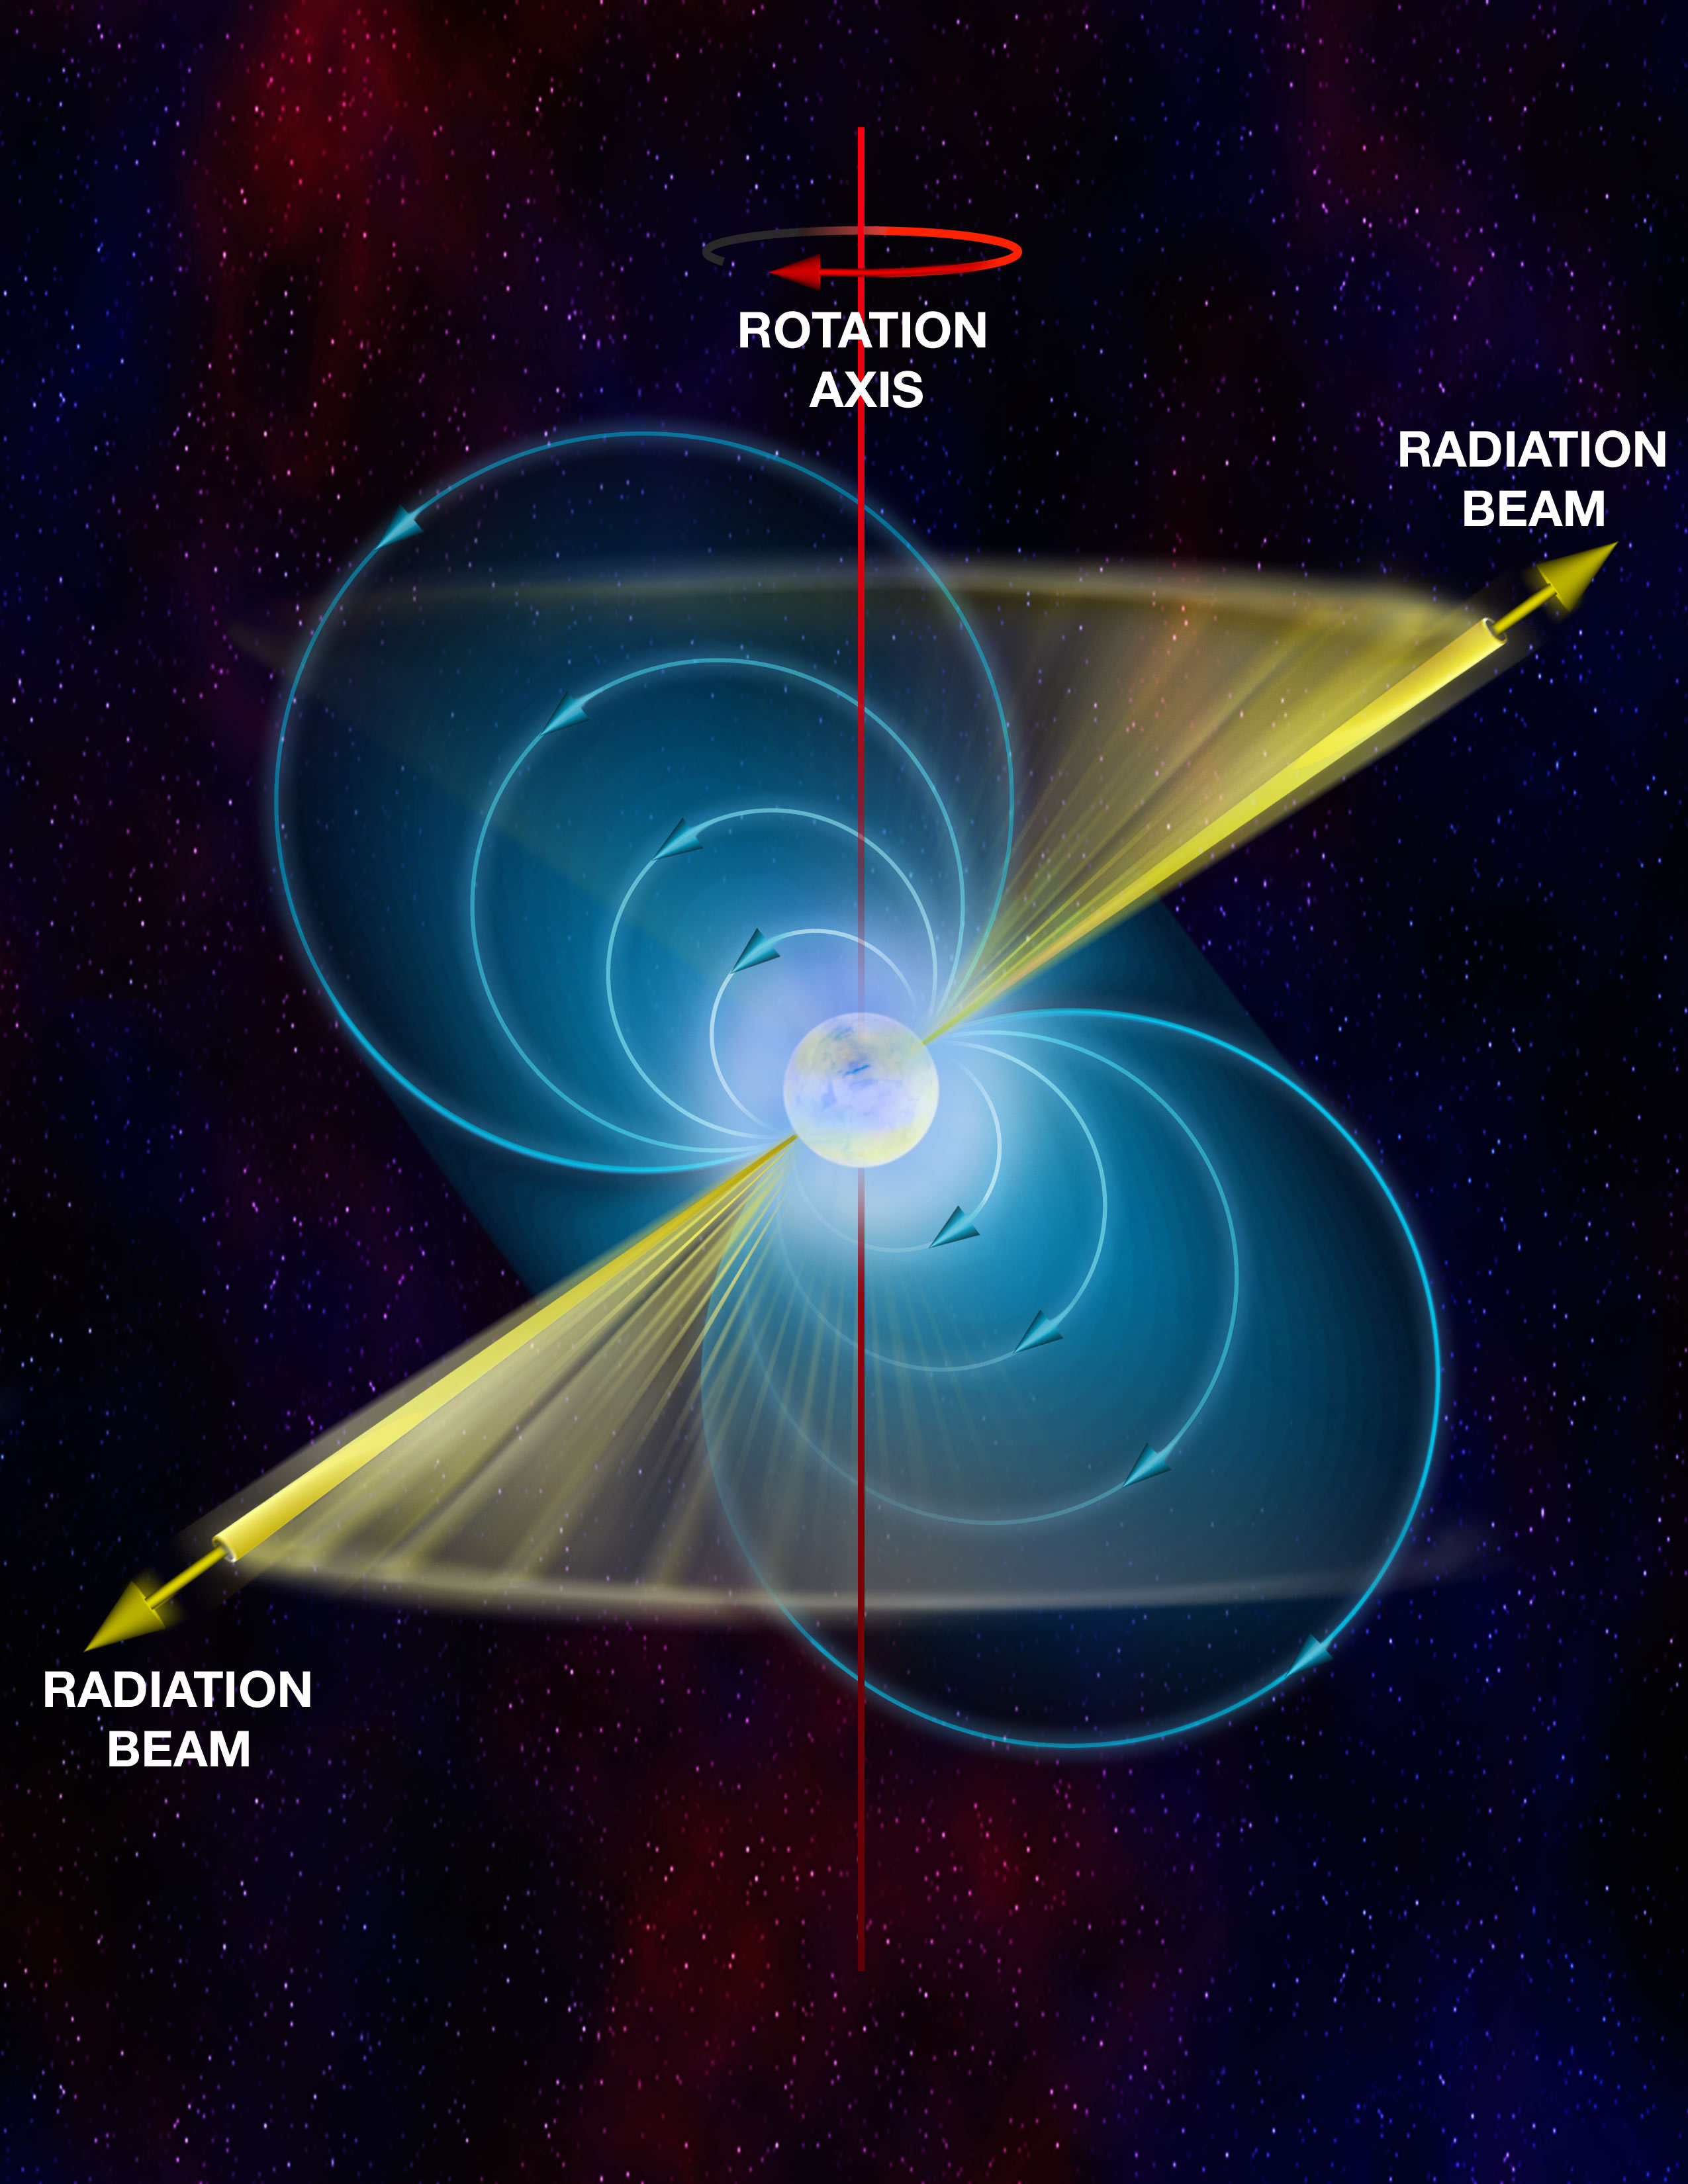
\includegraphics[scale=0.25]{Figures/pulsar.jpeg}
    \caption{Εκπομπή ακτινοβολίας από pulsar σύμφωνα με το πρότυπο εκπομπής από τους μαγνητικούς πόλους ενός αστέρα νετρονίων. Ο άξονας του μαγνητικού πεδίου δεν συμπίπτει με τον άξονα περιστροφής. Ένας παρατηρήτης βλέπει την ακτινοβολία από τον έναν πόλο μόνο.}
    \label{fig:pulsar}
\end{figure}

Το πιο διαδεδομένο πρότυπο για pulsars δέχεται ότι η περιοδική ακτινοβολία που παρατηρούμε έχει τη μορφή κωνικής δέσμης και προέρχεται από την περιοχή των μαγνητικών πόλων (polar cap model) ενός ταχέως περιστρεφόμενου αστέρα νετρονίων με ισχυρό \textit{διπολικό μαγνητικό πεδίο}. Η εξαιρετικά μικρή περίοδος περιστροφής των αστέρων νετρονίων και το ισχυρό μαγνητικό πεδίο τους οφείλονται, αντίστοιχα, στην διατήρηση της στροφορμής και της μαγνητικής ροής στην επιφάνεια του αρχικού αστέρα. Το εύρος της κωνικής δέσμης της ακτινοβολίας καθορίζεται από τη γωνιώδη απόσταση του τελευταίου \textit{ανοικτού σωλήνα μαγνητικής ροής} από το μαγνητικό άξονα του αστέρα. Επειδή ο μαγνητικός άξονας των pulsars δεν συμπίπτει συνήθως με τον άξονα περιστροφής τους, η κωνική δέσμη ακτινοβολίας του κάθε πόλου του pulsar σαρώνει έναν κοίλο κώνο με κορυφή τον pulsar. Αν η Γη τυχαίνει να βρίσκεται στο εσωτερικό του κοίλου κώνου, τότε σε κάθε περίοδο περιστροφής του αστέρα παρατηρούμε έναν παλμό ακτινοβολίας η διάρκεια του οποίου είναι ανάλογη προς το εύρος της κωνικής δέσμης. Η γεωμετρία αυτή θυμίζει το μηχανισμό της περιοδικής ακτινοβολίας ενός φάρου. 

Ο βασικός μηχανισμός ακτινοβολίας του παραπάνω προτύπου είναι ο εξής: το περιστρεφόμενο μαγνητικό πεδίο του αστέρα παράγει (εξ επαγωγής) διαφορά δυναμικού, όπως ακριβώς και οι γεννήτριες ηλεκτρικού ρεύματος, η οποία εμφανίζεται μεταξύ των πόλων και του ισημερινού του αστέρα. Λόγω αυτής της διαφοράς δυναμικού, φορτισμένα σωματίδια αποσπώνται από την επιφάνεια του αστέρα και δημιουργούν έναν τεράστιο ``πυκνωτή'' στην περιοχή του κάθε πόλου, οι οπλισμοί του οποίου αποτελούνται από δύο ετερόσημα στρώματα φορτίων: ένα στην επιφάνεια του pulsar και ένα στην περιοχή πάνω από αυτήν. Όταν η τάση μεταξύ των οπλισμών του κάθε ``πυκνωτή'' γίνει $10^{12} - 10^{13}\,\text{V}$, τότε επέρχεται εκφόρτισή τους. Η ενέργεια που παράγεται είναι πολύ μεγάλη (πολλές τάξεις μεγέθους μεγαλύτερη από $511\,\text{keV}$, που είναι η ισοδύναμη ενέργεια της μάζας ηρεμίας ενός ηλεκτρονίου) με αποτέλεσμα να συμβαίνει \textit{δίδυμη γέννηση} σωματιδίων (e$^{-}$- e$^{+}$). Τα σωματίδια αυτά κινούμενα ελικοειδώς γύρω από τις μαγνητικές δυναμικές γραμμές του πεδίου παράγουν ακτινοβολία \textit{σύγχροτρον} στην περιοχή των ραδιοφωνικών κυμάτων.

Το παραπάνω πρότυπο εξηγεί ικανοποιητικά τρία βασικά παρατηρησιακά δεδομένα των pulsars:
\begin{enumerate}
    \item Η δέσμη ακτινοβολίας είναι πολύ στενή, όπως προκύπτει από τους ``στενούς'' περιοδικούς παλμούς που παρατηρούμε. Η διάρκεια των μεμονομένων παλμών είναι της τάξης του 1/100 της περιόδου επανάληψης του παλμού (που, σύμφωνα με το πρότυπο, ισούται με την περίοδο περιστροφής του αστέρα).
    \item Το φάσμα της ακτινοβολίας των παλμών δεν μοιάζει με φάσμα μελανού σώματος, αλλά είναι φάσμα ακτινοβολίας σύγχροτρον.
    \item Οι παλμοί είναι πολύ ισχυρά γραμμικά πολωμένοι, γεγονός που απαιτεί ισχυρό μαγνητικό πεδίο.
\end{enumerate}

Υπάρχουν μερικοί pulsars που εκπέμπουν κυρίως στην περιοχή των ακτίνων-X. Οι pulsars αυτοί είναι μέλη ημιαποχωρισμένων διπλών συστημάτων (Κεφάλαιο \ref{ch:Chapter7}). Η ακτινοβολία τους, η οποία έχει φάσμα μελανού σώματος, εκπέμπεται από ύλη η οποία ``βομβαρδίζει'' την επιφάνεια του αστέρα και θερμαίνεται, πέφτοντας επάνω της με μεγάλη ταχύτητα (λόγω του ισχυρού βαρυτικού πεδίου του pulsar). Η ύλη αυτή προέρχεται από το συνοδό αστέρα, ο οποίος είναι συνήθως ένας εξελιγμένος (γίγαντας) αστέρας που έχει γεμίσει το λοβό Roche (δες Κεφάλαιο \ref{ch:Chapter7}).

Σήμερα πιστεύουμε ότι στο Γαλαξία υπάρχουν περίπου 50000 pulsars, ότι η δημιουργία τους συμβαίνει συνήθως κατά την έκρηξη ενός υπερκαινοφανούς αστέρα με ρυθμό περίπου ίσο με 1 pulsar ανά 20 έτη και ότι ο μέσος όρος ζωής τους είναι $10^7$ έτη. Ένας αστέρας νετρονίων παύει να παρατηρείται ως pulsar, είτε όταν το μαγνητικό του πεδίο εξασθενήσει σημαντικά, είτε όταν ο άξονας του (διπολικού) πεδίου γίνει παράλληλος προς τον άξονα περιστροφής. Και στις δύο περιπτώσεις το μέχρι σήμερα δεκτό πρότυπο ακτινοβολίας των pulsars (πρότυπο μαγνητικών πόλων) δεν προβλέπει περιοδική εκπομπή ακτινοβολιας.




% {\color{red} \hrule}
% Αστέρας νετρονίων είναι ο εκφυλισμένος, γυμνός πυρήνας ενός αστέρα με σχετικά μεγάλη αρχική μάζα. Η εξέλιξη της θερμοκρασίας του ακολουθεί, όπως πιστεύουμε σήμερα, την πορεία της θερμοκρασίας των λευκών νάνων. Σ' αυτήν την περίπτωση η υδροστατική ισορροπία εξασφαλίζεται από την κβαντομηχανικής φύσεως πίεσης των νετρονίων. Δεν αποκλείεται ενάς τέτοιος αστέρας να παρουσιαστεί ενεργά στον ουρανό υπό την μορφή ενός pulsar, που γίνεται ορατός με παρατηρήσεις σε ραδιαφωνικά, κυρίως, μήκη κύματος.\\
% {\color{red} \hrule}





\section{Μελανές οπές}
Η ύπαρξη ενός ανώτατου ορίου της μάζας ενός ευσταθή αστέρα νετρονίων δημιουργεί ένα δίλημμα. Όπως έχουμε ήδη αναφέρει, είναι γνωστό ότι υπάρχουν και αστέρες πολύ μεγάλης μάζας, που φυσικά είναι και οι ταχύτερα εξελισσόμενοι αστέρες. Προκύπτει, συνεπώς, το ερώτημα, τι θα συμβεί, αν α) ο αστέρας χάσει μεν κατά κάποιον τρόπο το μεγαλύτερο μέρος της μάζας του, αλλά η μάζα του παραμένοντος πυρήνα είναι μεγαλύτερη απο $2 - 3\,M_\odot$,  ή β) επιπρόσθετη μάζα πέσει πάνω σε έναν αστέρα νετρονίων, ώστε η μάζα του να υπερβεί την οριακή μάζα των $\sim 3\,M_\odot$. Στην περίπτωση αυτή δεν υπάρχουν γνωστές φυσικές δυνάμεις, ικανές να αναχαιτίσουν την ολοκληρωτική βαρυτική κατάρρευση του αστέρα. Συνεπώς, οι διαστάσεις του αστέρα συνεχώς σμικρύνονται και η ένταση του βαρυτικού πεδίου του αστέρα αυξάνει σε υπερβολικό βαθμό, οπότε, φυσικά, η χρήση της Γενικής Θεωρίας της Σχετικότητας είναι αναγκαστική. Η καμπύλωση του τετραδιάστατου χωροχρόνου του αστέρα δεν επιτρέπει ούτε καν φως να διαφύγει από το ισχυρότατο βαρυτικό πεδίο του και ο αστέρας φαίνεται να εξαφανίζεται από το σύμπαν. Το αποτέλεσμα αυτό της ολοκληρωτικής βαρυτικής κατάρρευσης έχει ονομαστεί \textit{μελανή οπή}.

Η δημιουργία μιας μελανής οπής ως αποτέλεσμα της ολοκληρωτικής βαρυτικής κατάρρευσης ενός αστέρα αποτελεί μια από τις πιο εντυπωσιακές προβλέψεις της Γενικής Θεωρίας της Σχετικότητας και της σύγχρονης θεωρίας της αστρικής εξέλιξης. Η ακριβής σχετικιστική περιγραφή του φαινομένου της βαρυτικής κατάρρευσης και των μαθηματικών ιδιοτήτων των μελανών οπών, φυσικά, δεν ανήκει στους αντικειμενικούς σκοπούς αυτών των σημειώσεων. Σε γενικές γραμμές, όμως, μπορούμε να πούμε, στην περίπτωση ενός σφαιρικά συμμετρικά αστέρα, οτι, αν η λόγω της βαρυτικής κατάρρευσης συνεχώς ελλατούμενη ακτίνα $R(R > R_s)$ του αστέρα πάρει την οριακή τιμή
$$R = R_s$$
ο αστέρας θα γίνει μη-ορατός για κάθε παρατηρητή. Τότε η εξωτερική (πραγματική) επιφάνεια του αστέρα γίνεται μια \textit{παγιδευμένη επιφάνεια} για υλικά σωματίδια και ακτίνες φωτός. Η επιφάνεια
\begin{equation}
	r = R_s = \frac{2GM}{c^2}
    \label{eq:schwarzschild_radius}
\end{equation}
ονομάζεται \textit{ορίζοντας γεγονότων} και ορίζεται από την ακτινική απόσταση που δίνεται από τη σχέση \eqref{eq:schwarzschild_radius} και που έχει ονομαστεί \textit{ακτίνα Schwarzschild}. Η μορφή της σχέσης αυτής προέκυψε από την σχέση \eqref{eq:escape_velocity} για $v_{\text{esc}} = c$, η απόδειξη όμως αυτή δεν είναι σωστή, επειδή οι σχέσεις της κλασικής φυσικής δεν ισχύουν στο εν λόγω όριο ταχύτητας.

Η σωστή απόδειξη δόθηκε από το Γερμανό αστροφυσικό Karl Schwarzschild το 1917, με βάση τη Γενική Θεωρία της Σχετικότητας. Ο Schwarzschild έδειξε ότι το μήκος κύματος ενός φωτονίου αυξάνεται, όταν αυτό απομακρύνεται από μία πηγή βαρυτικού πεδίου. Αν $\lambda_0$ είναι το μήκος κύματος σε απόσταση $r_0 > R_s$ από ένα ομογενές, σφαιρικό, μη-περιστρεφόμενο και ηλεκτρικά ουδέτερο σώμα με μάζα Μ και $\lambda$ είναι το μήκος κύματος σε άπειρη απόσταση από το σώμα, τότε ισχύει η σχέση
\begin{equation}
	\frac{\lambda}{\lambda_0} = \left( 1 - \frac{2GM}{r_0 c^2} \right)^{-1/2}
    \label{eq:black_hole_wavelength}
\end{equation}
Από τη σχέση \eqref{eq:black_hole_wavelength} βλέπουμε ότι, όταν το $r_0$ γίνει ίσο με $R_s$, τότε το $\lambda$ τείνει προς το $\infty$, η ενέργεια των φωτονίων $(E = h\nu = hc/\lambda)$ τείνει προς το μηδέν και επομένως αυτά παύουν να είναι αντιληπτά. Για το λόγο αυτό, αν ένα φωτόνιο περιέχεται μέσα σε σφαίρα ακτίνας $r \leq R_s$, τότε η τροχιά των φωτονίων στη θέση αυτή είναι κλειστή, και το φωτόνιο θα παραμείνει δέσμιο του βαρυτικού πεδίου. Η περιοχή $r < R_s$, λοιπόν, που περικλύεται από τον ορίζοντα γεγονότων είναι απαγορευμένη για έναν εξωτερικό παρατηρητή, με την έννοια ότι η έξοδος από αυτήν είναι αδύνατη (αν και η είσοδος σε αυτήν είναι δυνατή).

Ο ορίζοντας γεγονότων δεν είναι μία υλική επιφάνεια της μελανής οπής. Εντούτοις ένας εξωτερικός παρατηρητής που βρίσκεται σε απόσταση $r > R_s$ δεν μπορεί να πάρει άλλες πληροφορίες για την εσωτερική περιοχή $(r < R_s)$ παρά μόνο για την συνολική μάζα $(M)$, το ηλεκτρικό φορτίο $(Q)$ και την ολική στροφορμή $(J)$ που η περιοχή αυτή περιέχει. Αυτό συμβαίνει, επειδή οι παραπάνω ποσότητες σχετίζονται με το βαρυτικό και το ηλεκτρικό πεδίο, τα οποία είναι τα μοναδικά, γνωστά στη σημερινή Φυσική, πεδία, που συνδέονται με δυνάμεις μεγάλης ακτίνας δράσης (long range forces). 

Είναι φανερό ότι αν $r_0 \gg 2GM/c^2$, μπορούμε να αναπτύξουμε κατά Taylor το δεξιό μέλος της σχέσης \eqref{eq:black_hole_wavelength}, οπότε έχουμε
\begin{equation}
	\frac{\lambda_0}{\lambda} = 1 - \frac{GM}{r_o c^2}
\end{equation}
Αν πολλαπλασιάσουμε και τα δύο μέλη της εξίσωσης επί $E = hc/\lambda_0$ και θέοσυμε $m=E/c^2$, τότε βρίσκουμε ότι
\begin{equation*}
	h\nu = h\nu_0 - GMm/r_0
\end{equation*}
Η παραπάνω σχέση θυμίζει το ολοκλήρωμα της ενέργειας στο πρόβλημα των δύο σωμάτων
\begin{equation*}
	E_{\infty} = E_0 - GMm/r_0
\end{equation*}
Είναι φανερό ότι η ποσότητα $GMm/r_0$ αντιστοιχεί στην ενέργεια που καταναλώνει ένα φωτόνιο που βρίσκεται σε απόσταση $r_0$ από μία μάζα $M$ για να διαφύγει, σε άπειρη απόσταση, από την επίδραση της μάζας αυτής.

% {\color{red} \hrule}
% Στην περίπτωση των μελανών οπών, η υδροστατική ισορροπία του αστέρα έχει καταστραφεί, επειδή η διαθέσιμη πίεση (θερμικής ή κβαντομηχανικής προέλευσης) δεν είναι ικανή να αντισταθμίσει την βαρυτική. Η μάζα του αστέρα έχει καταρρεύσει, δημιουργώντας ένα αντικείμενο εξαιρετικά μεγάλης πυκνότητας. Σε κάθε μελανή οπή μπορούμε να αντιστοιχήσουμε ένα χαρακτηριστικό μήκος, $R_S$, που ονομάζεται ακτίνα Schwarzschild, με τη σχέση $R_S = 2GM/c^2$. Το βαρυτικό πεδίο μιας μελανής οπής είναι τόσο ισχυρό, ώστε σε απόσταση μικρότερη από την ακτίνα Schwarzschild ακόμα και το φως δεν μπορεί να διαφύγει από την βαρυτική έλξη.\\
% {\color{red} \hrule}

